% Arquivo LaTeX de exemplo de dissertação/tese a ser apresentados à CPG do IME-USP
% 
% Versão 5: Sex Mar  9 18:05:40 BRT 2012
%
% Criação: Jesús P. Mena-Chalco
% Revisão: Fabio Kon e Paulo Feofiloff
%  
% Obs: Leia previamente o texto do arquivo README.txt

\documentclass[11pt,twoside,a4paper]{book}

% ---------------------------------------------------------------------------- %
% Pacotes 
\usepackage[T1]{fontenc}
\usepackage[brazil]{babel}
\usepackage[utf8]{inputenc}
\usepackage[pdftex]{graphicx}           % usamos arquivos pdf/png como figuras
\usepackage{setspace}                   % espaçamento flexível
\usepackage{indentfirst}                % indentação do primeiro parágrafo
\usepackage{makeidx}                    % índice remissivo
\usepackage[nottoc]{tocbibind}          % acrescentamos a bibliografia/indice/conteudo no Table of Contents
\usepackage{courier}                    % usa o Adobe Courier no lugar de Computer Modern Typewriter
\usepackage{lmodern}                    % usa a versão amigável a caracteres acentuados da fonte Modern.
\usepackage{type1cm}                    % fontes realmente escaláveis
\usepackage{listings}                   % para formatar código-fonte (ex. em Java)
\usepackage{titletoc}
\RequirePackage{graphics}               % necessário para o clrscode3e
\usepackage{clrscode3e}                 % para formatar algoritmos como o CLRS
%\usepackage[bf,small,compact]{titlesec} % cabeçalhos dos títulos: menores e compactos
\usepackage[fixlanguage]{babelbib}
\usepackage[font=small,format=plain,labelfont=bf,up,textfont=it,up]{caption}
\usepackage[usenames,svgnames,dvipsnames]{xcolor}
\usepackage[a4paper,top=2.54cm,bottom=2.0cm,left=2.0cm,right=2.54cm]{geometry} % margens
\usepackage{tikz}
\usepackage{ifthen}
\usepackage{calc}
\usepackage{footnote}
\usepackage{amsmath}
\usepackage{amsfonts}
\usepackage[bottom]{footmisc}


%\usepackage[pdftex,plainpages=false,pdfpagelabels,pagebackref,colorlinks=true,citecolor=black,linkcolor=black,urlcolor=black,filecolor=black,bookmarksopen=true]{hyperref} % links em preto
\usepackage[pdftex,plainpages=false,pdfpagelabels,pagebackref,colorlinks=true,citecolor=DarkGreen,linkcolor=NavyBlue,urlcolor=DarkRed,filecolor=green,bookmarksopen=true]{hyperref} % links coloridos
\usepackage[all]{hypcap}                % soluciona o problema com o hyperref e capitulos
\usepackage[square,sort,nonamebreak,comma]{natbib}  % citação bibliográfica alpha (alpha-ime.bst)
\fontsize{60}{62}\usefont{OT1}{cmr}{m}{n}{\selectfont}

% ---------------------------------------------------------------------------- %
% Cabeçalhos similares ao TAOCP de Donald E. Knuth
\usepackage{fancyhdr}
\pagestyle{fancy}
\fancyhf{}
\renewcommand{\chaptermark}[1]{\markboth{\MakeUppercase{#1}}{}}
\renewcommand{\sectionmark}[1]{\markright{\MakeUppercase{#1}}{}}
\renewcommand{\headrulewidth}{0pt}

% ---------------------------------------------------------------------------- %
\graphicspath{{./figuras/}}             % caminho das figuras (recomendável)
\frenchspacing                          % arruma o espaço: id est (i.e.) e exempli gratia (e.g.) 
\urlstyle{same}                         % URL com o mesmo estilo do texto e não mono-spaced
\makeindex                              % para o índice remissivo
\raggedbottom                           % para não permitir espaços extra no texto
\fontsize{60}{62}\usefont{OT1}{cmr}{m}{n}{\selectfont}
\cleardoublepage
\normalsize

% ---------------------------------------------------------------------------- %
% Opções de listing usados para o código fonte
% Ref: http://en.wikibooks.org/wiki/LaTeX/Packages/Listings
\lstset{ %
language=Java,                  % choose the language of the code
basicstyle=\footnotesize,       % the size of the fonts that are used for the code
numbers=left,                   % where to put the line-numbers
numberstyle=\footnotesize,      % the size of the fonts that are used for the line-numbers
stepnumber=1,                   % the step between two line-numbers. If it's 1 each line will be numbered
numbersep=5pt,                  % how far the line-numbers are from the code
showspaces=false,               % show spaces adding particular underscores
showstringspaces=false,         % underline spaces within strings
showtabs=false,                 % show tabs within strings adding particular underscores
frame=single,	                % adds a frame around the code
framerule=0.6pt,
tabsize=2,	                    % sets default tabsize to 2 spaces
captionpos=b,                   % sets the caption-position to bottom
breaklines=true,                % sets automatic line breaking
breakatwhitespace=false,        % sets if automatic breaks should only happen at whitespace
escapeinside={\%*}{*)},         % if you want to add a comment within your code
backgroundcolor=\color[rgb]{1.0,1.0,1.0}, % choose the background color.
rulecolor=\color[rgb]{0.8,0.8,0.8},
extendedchars=true,
xleftmargin=10pt,
xrightmargin=10pt,
framexleftmargin=10pt,
framexrightmargin=10pt
}




% ---------------------------------------------------------------------------- %
% Corpo do texto
\begin{document}
\newcommand{\ttt}[1]{\texttt{#1}}

\frontmatter 
% cabeçalho para as páginas das seções anteriores ao capítulo 1 (frontmatter)
\fancyhead[RO]{{\footnotesize\rightmark}\hspace{2em}\thepage}
\setcounter{tocdepth}{2}
\fancyhead[LE]{\thepage\hspace{2em}\footnotesize{\leftmark}}
\fancyhead[RE,LO]{}
\fancyhead[RO]{{\footnotesize\rightmark}\hspace{2em}\thepage}

\onehalfspacing  % espaçamento



% ---------------------------------------------------------------------------- %
% Resumo

% CAPA
% Nota: O título para as dissertações/teses do IME-USP devem caber em um 
% orifício de 10,7cm de largura x 6,0cm de altura que há na capa fornecida pela SPG.
\thispagestyle{empty}
\begin{center}
    \vspace*{2.3cm}
    \textbf{\Large{ Predição do impacto do fluxo de dados no desempenho de workflows científicos}}\\
    
    \vspace*{1.2cm}
    \Large{Duílio Henrique Haroldo Elias}
    \vskip 1.5cm  
    \textsc{Relatório Parcial de Iniciação Científica}
      		
    \vskip 1.5cm
    Programa: Programa Institucional de Bolsas de
Iniciação Científica em Desenvolvimento Tecnológico e Inovação – PIBITI/CNPq/USP\\
    Orientadora: Kelly Rosa Braghetto\\
   	\vskip 1cm
   	
   	Departamento de Ciências da Computação\\Instituto de Matemática e Estatística\\Universidade de São Paulo
     \vskip 0.5cm
    \normalsize{\today}
\end{center}
% Retira espaço extra obsoleto entre as frases.
\frenchspacing 
\newpage
% ----------------------------------------------------------
% ELEMENTOS PRÉ-TEXTUAIS
% ----------------------------------------------------------
% resumo em português
\begin{resumo}

	Nas últimas décadas os workflows científicos receberam grande atenção da comunidade acadêmica, devido à sua grande capacidade de manipulação, análise e simulação de experimentos que trabalham com grandes quantidades de dados. No entanto, as ferramentas existentes para tal fim são ainda escassas e muitos cientistas afirmam que isso seja o grande gargalo da produção científica. Neste trabalho, busca-se contribuir com este processo, a partir da identificação e caracterização de linguagens de modelagem de workflows científicos, criando modelos estocásticos capazes de predizer o impacto causado pelo fluxo de dados no desempenho e na execução de workflows em ambientes computacionais distribuídos. Com isso, pretende-se desenvolver um algoritmo que gera modelos estocásticos a partir do fluxo de dados de workflows científicos, extraindo índices capazes de predizer o impacto do uso de diferentes abordagens de controle de fluxo de dados no desempenho dos workflows.

 \vspace{\onelineskip}
 
 \noindent
 \textbf{Palavras-chaves}: Workflows científicos. Redes de Petri. Análise de Desempenho. Gerenciadores de Workflows.
\end{resumo}
\newpage

% ---
% inserir o sumario
% ---
\pdfbookmark[0]{\contentsname}{toc}
\tableofcontents*
\cleardoublepage
% ---
% ----------------------------------------------------------
% ELEMENTOS TEXTUAIS
% ----------------------------------------------------------
\textual
% ----------------------------------------------------------
% Introdução
% ----------------------------------------------------------

\section{Introdução}

%definicao e caracteristicas básicas de workflows cientificos OK
%colocar uma idea de redes de petri estocásticas

	Um workflow científico\cite{alkmin:migracao_maquinas_virtuais} pode ser compreendido como um conjunto de tarefas computacionais que constituem um experimento científico[Referenciar texto/encontrar outra definição]. Esse conjunto de tarefas pode ser dividido em modelagem, execução e análise. Um cientista pode definir seu workflow com o auxílio de uma ferramenta de software, com uma interface gráfica simples e intuitiva. Depois de criado um modelo, o gerenciador auxilia o pesquisador a executar o workflow de forma eficiente, automaticamente, com pouca ou nenhuma intervenção manual.
	
	Os workflows científicos são conhecidos pelo seu poder de manipulação e execução de projetos que trabalham com grandes quantidades de dados. Neste trabalho, estamos interessados em melhorar o desempenho da execução de workflows em ambientes computacionais distribuídos, o que muitas vezes não é uma tarefa fácil. Para isso, o sistema gerenciador precisa considerar a relação de dependência que existe entre as tarefas do workflow, ou seja, precisa definir quais são os dados de entrada de uma determinada tarefa, a fonte desses dados e destino dos dados processados. Há também um custo envolvido nas transferências de dados, em termos de tempo, que precisa ser considerado e que depende do ambiente computacional.

	Todas essas observações se relacionam ao modelo de workflow de duas formas diferentes: primeiro, pela relação de dependência existente entre as tarefas, ou seja, como os dados irão percorrer o workflow e, segundo, quais as características computacionais do ambiente em que o workflow será executado.
	
	O conjunto de conexões que interligam as atividades pode ser caracterizado como fluxo de dados, esse fluxo de dados define as dependências entre as atividades e os dados manipulados[Texto Eduardo].


	
	%colocar a importacia da analise do fluxo de dados para extrair índices de desempenho.
	%colocar aqui algumas palavras sobre a modelagem analítica e sobre redes de Petri
	
\section{Objetivo}

		Neste trabalho, pretende-se identificar e caracterizar os principais construtores de fluxo de dados encontrados em linguagens de modelagem de workflows científicos, bem como criar modelos estocásticos em Redes de Petri capazes de predizer o impacto causado pelo fluxo de dados no desempenho da execução de workflows. Para validar os índices que espera-se obter do modelo estocástico criado, serão modelados em Redes de Petri um conjunto de workflows científicos bem conhecidos pela comunidade científica, como o Montagem\footnote{https://confluence.pegasus.isi.edu/display/pegasus/Montage+Characterization}. As predições obtidas a partir do modelo de Redes de Petri são comparadas com as obtidas a partir da simulacão da execucão dos mesmos workflows na ferramenta de simulacão CloudSim-DVFS.
		Com as experiências obtidas nas fases anteriores pretende-se criar um algoritmo capaz de gerar modelos estocásticos a partir de modelos de fluxos de dados de workflows científicos.

% ----------------------------------------------------------
% Seção de explicações
% ----------------------------------------------------------

\section{Conceitos Preliminares}
	%colocar definicao de workflows e diferença entre workflows de negocio e 		cientificos. OK
	%Tipos de fluxos de dados OK		
	\subsection{Workflows científicos}
		
		O termo workflow tem sua origem ligada a processos de automação de escritórios  que surgiram na década de 70. Com o objetivo de de gerar uma tecnologia capaz de fornecer uma base de apoio à distribuição de documentos nos escritórios, o que resultou na diminuição do uso de papéis[(Hollingsworth 1995, Mattos et al.2008)]. Embora a sua origem esteja mais relacionada com a automação de tarefas de logística, essa teoria foi expandida para outras áreas do conhecimento, como Economia, Administração, até mesmo Física, Biologia e Oceanográfica. Segundo \textit{Workflow Management Coalition}[referênciar], um workflow pode ser definido como: "A automação de um processo de negócio, completo ou apenas parte dele, através do qual documentos, informações ou tarefas são transmitidos de um participante a outro por ações, de acordo com regras procedimentais".

		Já o termo workflow científico está bem mais ligado com as ciências do que o termo workflow, por ter o seu foco na manipulação de dados e na execução de tarefas que estão diretamente relacionadas com o processamento de dados. Essa grande utilização de dados caracteriza os workflows científicos como uma estrutura baseada no fluxo de dados, ou seja, as conexões entre as atividades representam o fluxo de dados.[referenciar texto Eduardo]
		 
		Os sistemas de workflows científicos geralmente são compostos por um grande número de tarefas que podem depender dos dados produzidos por outras tarefas. Essas tarefas podem ser manuais ou automáticas e são responsáveis pela gerência de todo o ciclo de vida do experimento científico: composição, mapeamento, execução e análise. Cada etapa do ciclo do experimento é muito importante e precisa ser analisada com cuidado[Referenciar texto Doc1]:

	\begin{itemize}
		\item Composição: especificações das tarefas que compõem o experimento, dos tipos de dados de entrada e saída e das dependências de dados existentes entre as atividades e o ambiente computacional em que o workflows será executado.
		
		\item Mapeamento: associação do modelo de workflow com os recursos computacionais disponíveis.		
		
		\item Execução: realização das tarefas definidas anteriormente no ambiente computacional.

		\item Análise: estudo dos dados gerados na execução.

	\end{itemize}


		Todo esse processo pode ser automatizado de forma que o cientista possa reexecutá-lo até que os dados obtidos na fase de análise sejam os dados esperados. 
		
		A estrutura de um workflow é composta pelas atividades a serem executadas e as conexões entre elas. Compreende-se por atividade cada ação realizada que recebe um dado de entrada e produz um dado ou uma informação de saída. O conjunto de conexões entre as atividades pode ser caracterizado como fluxo de controle ou fluxo de dados. Neste trabalho estamos interessados em analisar apenas o fluxo de dados, pois é a estrutura que está mais interligada com os workflows científicos . O fluxo de dados representa a dependência entre as atividades e os dados manipulados, e a forma como os dados são utilizados no workflow, com atividades produzindo dados que serão consumidos por outras atividades[Qualificação eduardo]. 

		As principais construções de fluxo de dados são:[Texto eduardo]:
		
	\begin{itemize}
		\item \textit{Pipeline}: são várias atividades combinadas sequencialmente, em que cada atividade recebe como entrada os dados produzidos como saída da atividade anterior;  

		\item \textit{Distribuição de dados}: é feita por atividades que produzem dados de saída que são recebidos como entrada por múltiplas atividades, ou que apenas particionam grandes conjuntos de dados em subconjuntos menores para serem processadas por outras atividades;
		
		\item \textit{Agregarão de dados}: é feita por atividades que processam múltiplos conjuntos de dados de entrada, gerando uma combinação dos dados como saída;
		
		\item \textit{Redistribuição de dados}: é feita por atividades que funciona como um ponto de sincronização com relação ao processamento de dados, recebendo como entrada várias porções de dados e produzindo também múltiplas saídas como resultado.
	\end{itemize}
		
	Todas essas construções serão exemplificadas graficamente na seção[X], descritos simplificadamente a seguir.
			
		%caractericao geral dos gerenciadores kepler, taverna.
		%falar depois do Pegasus e do DAX que utilizado pelo pegasus, o motagem é feito em cima do formato DAX.
		\subsection{Sistemas gerenciadores de workflows científicos}
				
			\subsubsection{Kepler}
				
				
			\subsubsection{Taverna}
				O Taverna foi desenvolvido como parte do projeto \textit{mygrid}\footnote{http://www.mygrid.org.uk/}, é um ambiente para modelagem, execução e análise de workflows científicos, tem como foco principal aparar cientistas da área de Ciências Biológicas que normalmente não possuem conhecimento profundo de computação. O Taverna tem código aberto o que permite unir projeto de terceiros[Referenciar texto eduardo].

				Um workflow no Taverna é especificado como um grafo direcionado onde os nós, chamados de processadores,  são as atividades e representam componentes de software. Um nó processador consome dados que chegam nas suas entradas e produzem dados de saída. Cada arco no grafo conecta um entrada com uma saída de dados e expressa uma dependência entre as atividades o que denota o fluxo de dados entre as atividades.
				
				A construção e execução dos workflows no Taverna é feita com o auxilio de uma interface gráfica e depois é representado em uma linguagem baseada em XML e depois é executado pelo \textit{motor de execucão}. Observe a seguir uma imagem desse interface gráfica:
				
		\begin{figure}[!h]
			\centering
			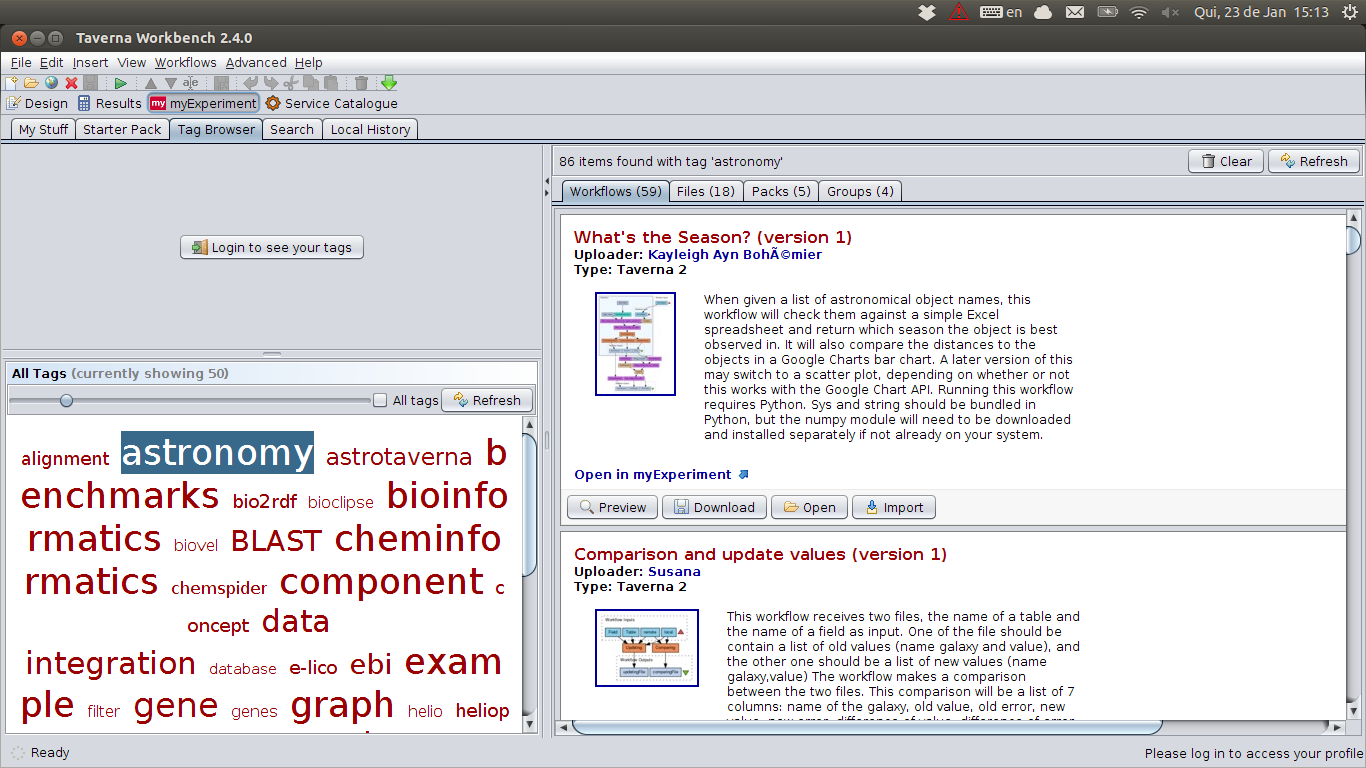
\includegraphics[scale=0.3]{img/taverna.png}
			\caption{Interface gráfica do Taverna}
		\end{figure}
		
		O \textit{myexperiemente}\footnote{http://www.myexperiment.org/} visto na figura é um repositório onde a comunidade compartilha seus workflows.
		
		O fluxo de dados no Taverna pode ser gerenciado a partir da sua interface gráfica e construção de \textit{pipelines} é a sua construção mais básica. Mas é possível criar construções como Agregação,Distribuição e Redistribuição de dados. 
		
		
		%colocar a definicao formal de redes de Petri, pegar na dissertacao da professra Kelly		OK
	\subsection{Redes de Petri}
		As Redes Petri(RdP) é um dos formalismos mais utilizados para modelagem analítica e análise de sistemas concorrentes mais utilizados,isso deve-se à fácil compreensão representação gráfica e devido ao seu potencial matemático para análise de modelos. Algumas características importantes de workflows científicos pôde ser facilmente representadas utilizando RdP, tais como a sincronização de tarefas, concorrência e controle de dependências[Referencia dissertação kelly].
		Uma RdP pode ser formalmente definida pela tupla $RdP={L,T,A,P,m_{0}}$, em que:
		\begin{itemize}
		\item $L=\{l_{1},l_{2},...,l_{L}\}$ é um conjunto de lugares;
		\item $T=\{t_{1},t_{2},...,t_{T}\}$ é um conjunto de transições;
		\item $A\subseteq(L x T)\bigcup (TxL)$ é um conjunto de arcos;
		\item $P: A \rightarrow \mathbbm{N}$ é a função peso dos arcos;
		\item $m_{0}=\{m_{01},m_{02},...,m_{0L}\}$ é a marcação inicial da rede;
		\end{itemize}
		
		Cada um dessas definições está associados a diferentes e importantes conceitos de RdP, que são:
		
			\begin{itemize}

				\item \textit{lugar} (representado graficamente por um círculo)- modela uma condição que deve ser satisfeita para que o disparo da transição seja realizado;

				\item \textit{transição} (representado graficamente por um retângulo) - pode ser compreendido por uma por uma acao ou um evento;

				\item \textit{arco orientado} liga um lugar a uma transição ou o contrário, ligando condições e eventos;

				\item \textit{fichas, marcas ou tokens} (representado por um ponto preto)- Representam um recurso ou um estado de um sistema;

				\item \textit{peso} - os arcos possuem um peso associado a eles; os pesos indica quantas fichas uma transição consome de um lugar de entrada ou quantas fichas uma transição acrescenta em um lugar de saída. Por \textit{default} quando um arco não possui um peso o peso é 1;
					
			\end{itemize}
			
			Da necessidade de modelagem de sistemas grandes e complexos, como os encontrados na natureza e na sociedade, foram definidas sobre a base de Redes de Petri clássica outras redes de alto nível, como as Redes de Petri Temporizadas(RdPTs) e Redes de Petri Estocásticas(RdPEs). As RdPTs como o nome diz permite modelar situações que ocorrem entre o início e fim de cada tarefa em termos do tempos. O permitiu diferentes possibilidades para modelagem, como lugares temporizados, fichas temporizadas e todas as outras estruturas descritas acima puderam ser tempodizadas e permitiram modelar uma série de sistemas reais. Já as RdPEs é uma subclasse das RdPTs, onde o tempo de atraso de uma transição é uma variável aleatória exponencialmente distribuída[Referenciar Kelly].
			%mostra como podemos aplicar redes de Petri na modelagem analitica de workflows cientificos
			%relacionar modelage analítica de redes de Petri com workflows científicos	
			%colocar porque escolhermos esse formalismo em vez de outros N/D
			\subsubsection{Introdução à modelos estocásticos para avaliação preditiva de desempenho de workflows científicos}

				Neste trabalho, a análise de desempenho de workflows científicos baseia-se em duas abordagens diferentes: primeiro, uma modelagem analítica, apoiando-se no formalismo estocástico de redes de Petri, segundo, a simulação dos workflows científicos no [CloudSim-DVSF]. Essas duas fases permitirá extrair e comparará-los.
				
				 
		%colocar aqui como será modelado as redes de Petri para criar uma rede similar ao workflow analisado
		\subsection{Modelagem e representação de fluxos de dados}	
		\subsection{Simuladores de workflows científicos}	
				
				Depois de criados os modelos em RdPEs para workflows científicos há algumas maneiras de validar o modelo, a primeira possibilidade é execução do workflows. Essa alternativa possui como problema o custo monetário envolvido na instanciação das máquinas, o que a torna inviável no primeiro momento. Uma outra alternativa mais viável é a  utilização de um ambiente de simulação computacional. Essa alternativa abre a possibilidade de criar-se diferentes ambientes computacionais e facilidade de reprodução da simulação, o que torna viável a busca por gargalos no workflows utilizados.
		\subsubsection{CloudSim}
			O 
				
				
				
		%Para extrair índices de desempenho precisamos primeiro ter a solucao numerica do modelo, existem varias 				ferramentas para a modelagem de redes de Petri estocasticas e escolhemos utilizar a PIPE, ferramenta open source 		...
	% Para validar o índices de desempenho que serão extraidos na proxima fase do projeto, foram estudados alguns também 	simuladores, falar sobre o workflow_sim e cloud-sim_DVSF. No simulador é possível modelar o ambiente computacional 	e para avaliar a posteriore teremos que modelar esse ambiente computacional utilizando redes de Petri.
	%Falar sobre o DAX;caracterizar um workflow descrito por DAX e da possibilidade de converter um workflow em DAX em 	modelo analítico. Pegar um exemplo simples e colocar no relatório.
%Como foram realizadas as tarefas 

\section{Metodologia}

		%colocar a possibilidades de construcao do ambiente computacional na nuvem.
		Para a modelagem analítica com RdPEs optou-se pelo uso da Ferramenta PIPE \footnote{http://pipe2.sourceforge.net/} e para a simulação utiliza-se o CouldSim-DVFS. Todos esses Softwares serão descritos e aplicados nas próximas seções.
	
	
	%Depois do estudo de workflows científicos e suas características, para se extrair índices de desempenho dos workflows científicos e ter possibilidade de ser criar no futuro um algoritmo capaz de modelar analiticamente um workflow simples no forma DAX precisamos conhecer a estrutura de comportamento dos fluxo de dados dos workflows e caracterizar esse fluxo de dados extrair em alguns padrões de comportamento % colocar as possibilidades de fluxo de dados 
	%Assim modelamos em Redes de Petri um workflow bem conhecido pela conhecido pela comunidade o montagem como pode ser visto da figura abaixo:

	%Observe que apareceram algumas estruturas para modelar em Redes de Petri o Montage, isso mostra o poder dessa teoria em modelagem analítica de workflows científica, como foi visto acima com redes de Petri é possível criar sincronização, paralelismo...[Continuar depois]
	%Isso permitirá no futuro extrai-se índices de desempenho, a partir da modelagem analítica de alguns workflows científicos e com isso há a possibilidade de validar esses índices com o auxilio dos simuladores descritos acima, ou seja, no simulador é possível espera-se criar um ambiente computacional análogo ao ambiente disponível para a execucão do workflow.
	
%A partido dos estudos... é possível automatizar a conversão de de modelos em DAX, sem grandes problemas.

\section{Resultados Parciais}
	Assim, pode-se ter uma comparação entre os modelos analíticos, a simulação e o experimento real.
	O que servirá a posteriore para extrair índices de desempenho e criar um algoritmo capaz de encontrar a melhor forma de modelagem do workflow científico.
%Quais os critérios que utilizaremos para criar correcoe?
	
	%Falar sobre o sucesso da atividades que nos compromentemos e sobre o que pretendemos fazer depois(Fazer a 				programa conversão automatica e modelar um ambiente computacional com redes de Petri, definir um método de 			extracao de índices de desempenho, a partir da solucao matemática de um modelo em redes de Petri).


\section{Conclusões Parciais}

\begin{figure}[!h]
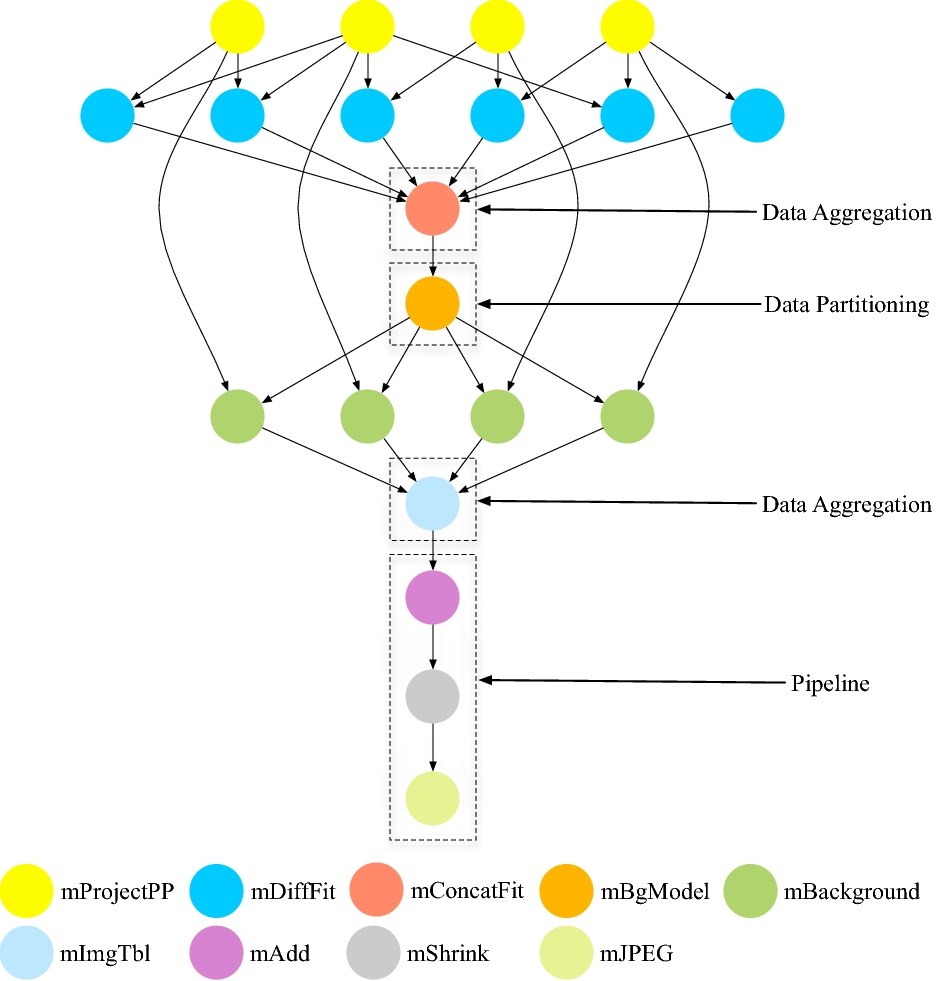
\includegraphics[scale=0.3]{img/Montage.jpg}
\end{figure}


\begin{figure}[h]
		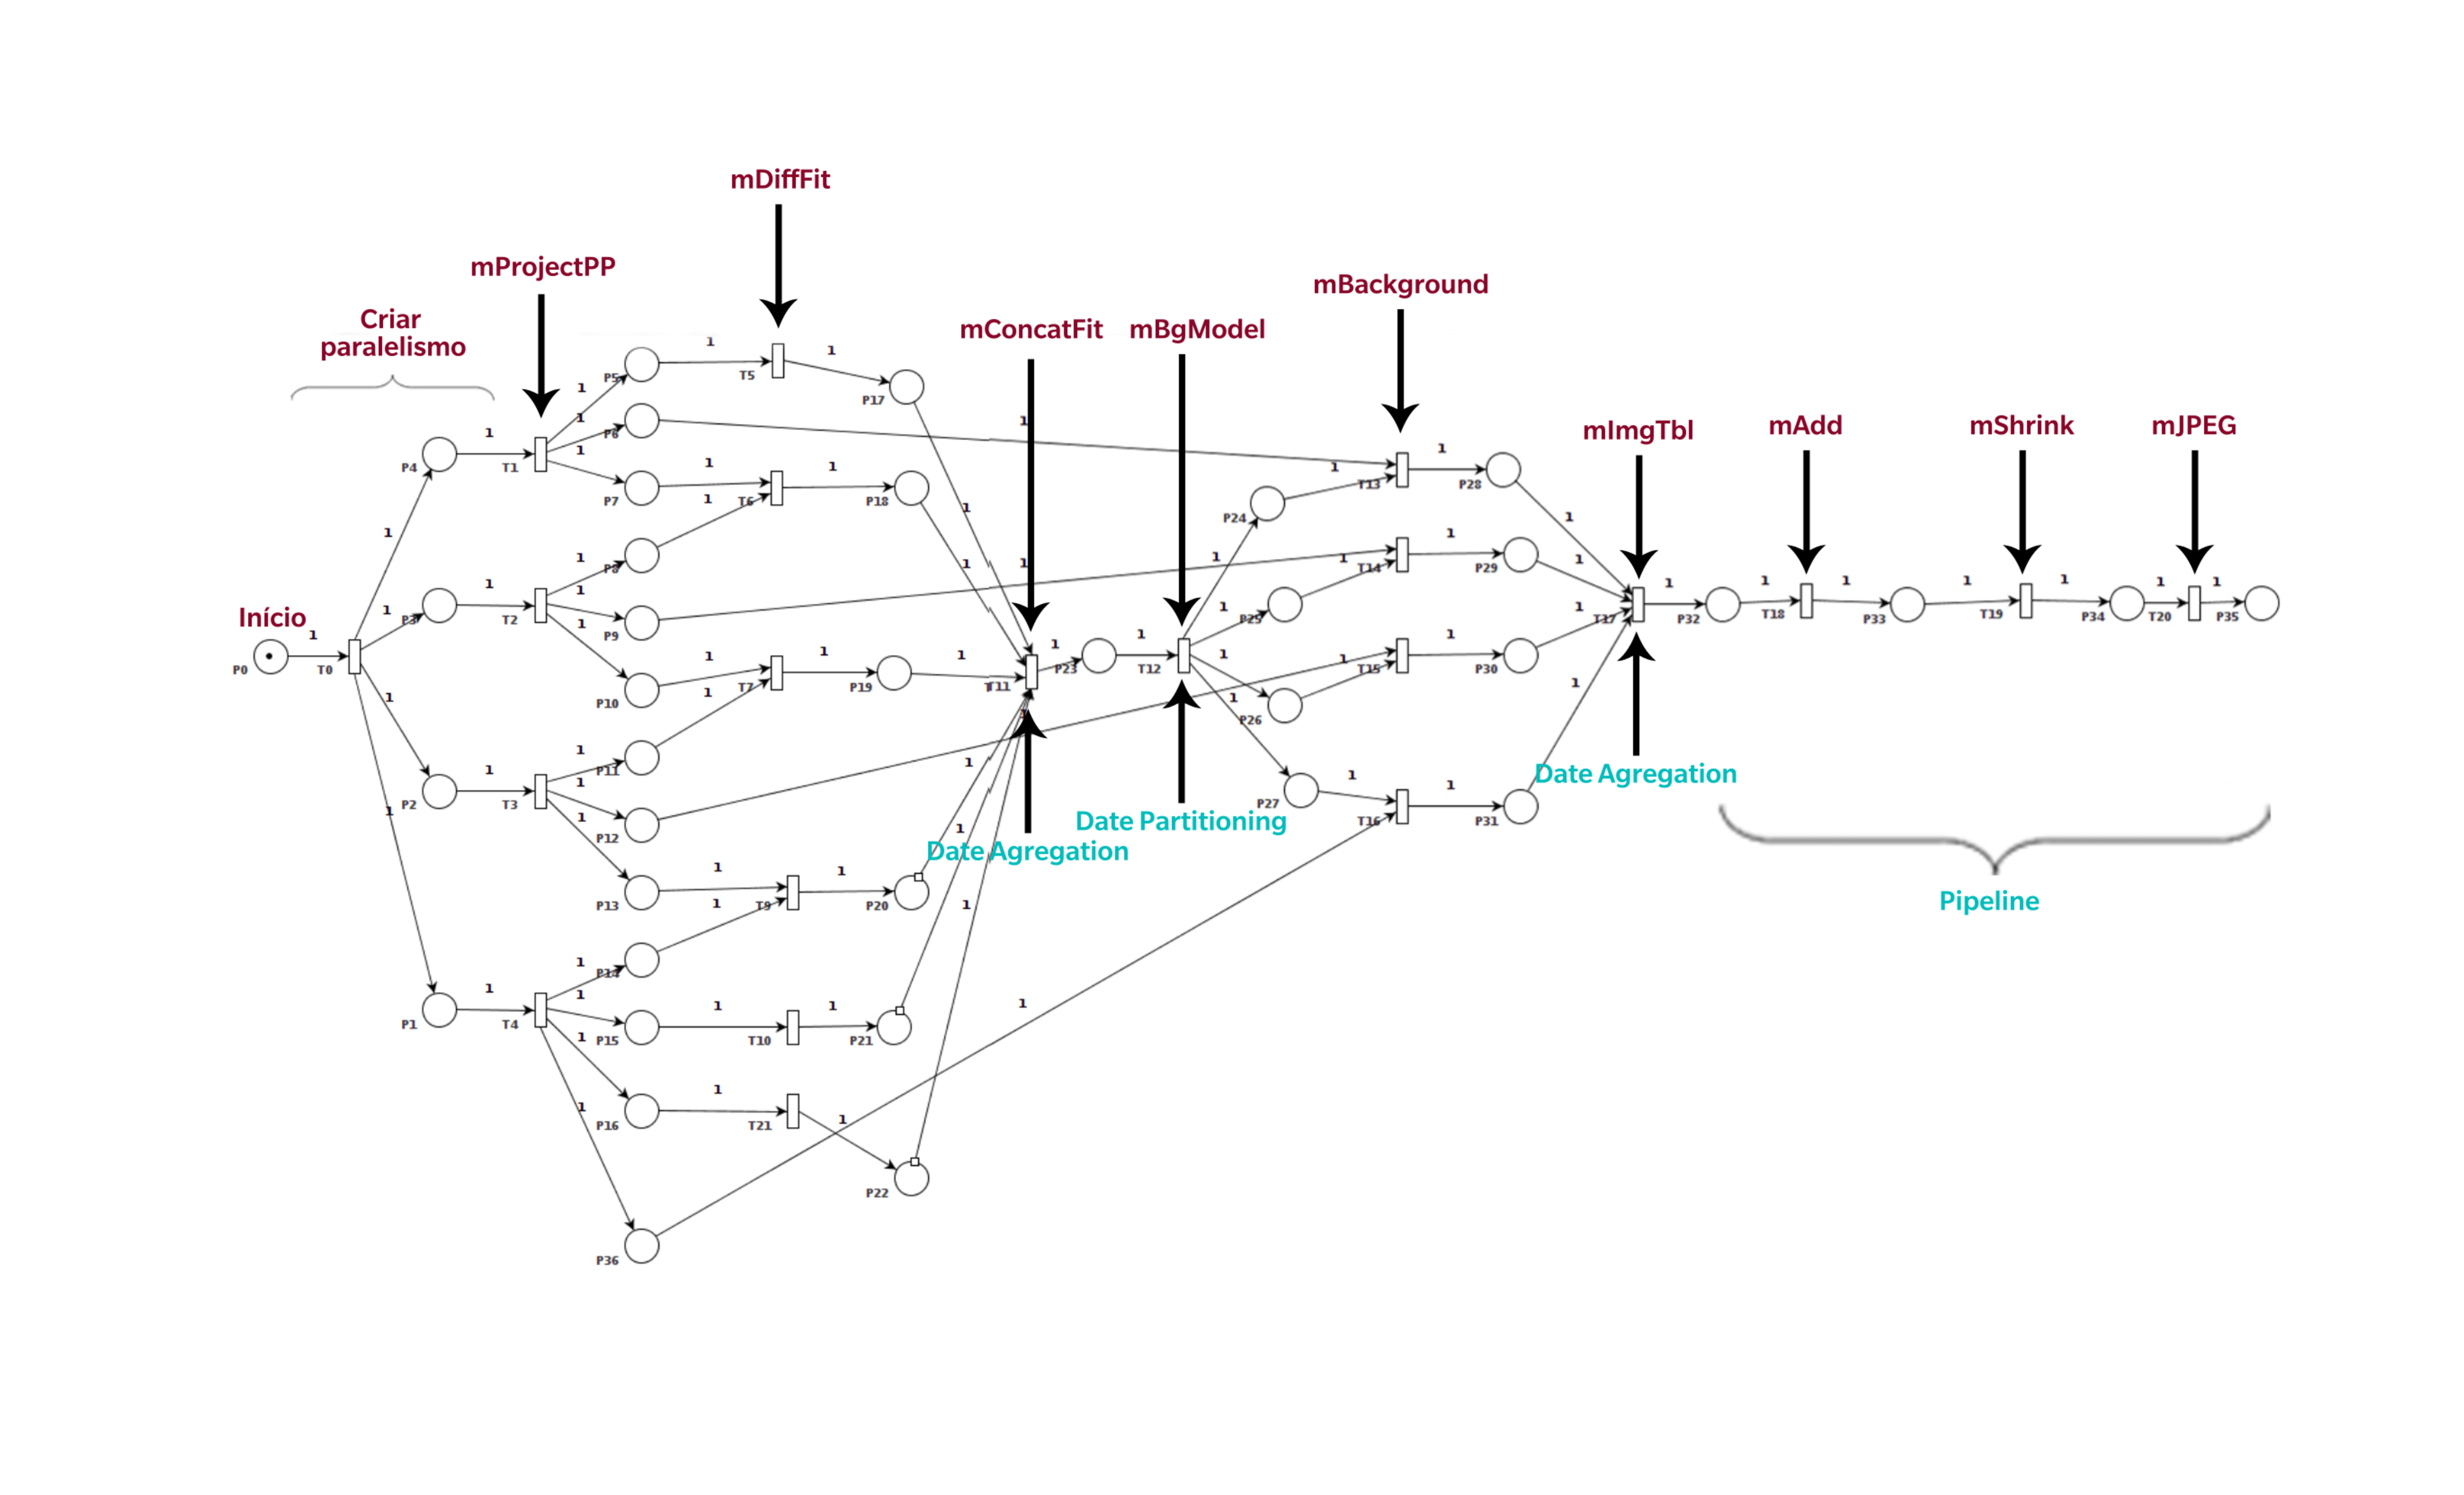
\includegraphics[scale=0.2]{img/RP_montage.pdf}
\end{figure}


\part{Parte Objetiva}

\input cap-cronograma        % associado ao arquivo: 'cap-cronograma.tex'
\input cap-introducao        % associado ao arquivo: 'cap-introducao.tex'
\input cap-conceitos         % associado ao arquivo: 'cap-conceitos.tex'
\input cap-experimentos      % associado ao arquivo: 'cap-experimentos.tex'
\input cap-conclusoes        % associado ao arquivo: 'cap-conclusoes.tex'

\part{Parte Subjetiva}

\input cap-o-tcc             % associado ao arquivo: 'cap-o-tcc.tex'
\input cap-a-graduacao       % associado ao arquivo: 'cap-a-graduacao.tex'

% cabeçalho para os apêndices
%\renewcommand{\chaptermark}[1]{\markboth{\MakeUppercase{\appendixname\ \thechapter}} {\MakeUppercase{#1}} }
%\fancyhead[RE,LO]{}
%\appendix

%\include{ape-conjuntos}      % associado ao arquivo: 'ape-conjuntos.tex'

% ---------------------------------------------------------------------------- %
% Bibliografia
\backmatter \singlespacing   % espaçamento simples
\bibliographystyle{alpha-ime}% citação bibliográfica alpha
\bibliography{bibliografia}  % associado ao arquivo: 'bibliografia.bib'

% ---------------------------------------------------------------------------- %
% Índice remissivo
%\index{TBP|see{periodicidade região codificante}}
%\index{DSP|see{processamento digital de sinais}}
%\index{STFT|see{transformada de Fourier de tempo reduzido}}
%\index{DFT|see{transformada discreta de Fourier}}
%\index{Fourier!transformada|see{transformada de Fourier}}

%\printindex   % imprime o índice remissivo no documento 

\end{document}
